\chapter{Implementation} \label{implementation}

\section{RTAB-Map}

For the appropriate usage of RTAB-Map~\cite{RTAB_Map_docs} we had to modify its launch files. Our goal was to start the camera on the robot (because it is attached to it), then publish the images and IMU data onto a ROS topic which can be processed by the notebook on top.

When we start the \verb|rtabmap.launch.py| launch file inside the \verb|depthai_ros_driver| package it automatically starts the camera's node in addition to the RTAB-Map node. It was not ideal for us since the camera node should run on the robot and the RTAB-Map (which requires more computation resources) on the notebook. Our solution was to create a new launch file (which can be examined at \ref{rtabmap_custom_launch_file}) based on \verb|rtabmap.launch.py| which starts everything but the camera node. With the help of this we can launch RTAB-Map on the notebook without the camera. The camera can be started on the robot with the basic \verb|camera.launch.py| launch file from the \verb|depthai_ros_driver| package. A mapping made with this approach can be seen on Figure~\ref{fig:rtabmap_nokia}.

\section{Person detection}

For the person detection we first tried out the Spectacular AI's example on the robot's camera but we soon realised that the position of it is not ideal for detecting objects. Due to the platform above the robot it limits the FOV (Field of View) of the camera so much that if we stood 2-3 meters away from the robot only our legs were visible thus the detection was not working. Our solution for this problem was to put the camera right at the front of the platform with some plasticine and it worked because the FOV increased a lot. The detection of my advisor with the camera at front can be seen on Figure \ref{fig:person_detection_camera_at_front_nokia} (the other detected person is a woman on a poster).

\begin{figure}[htbp]
    \centering
    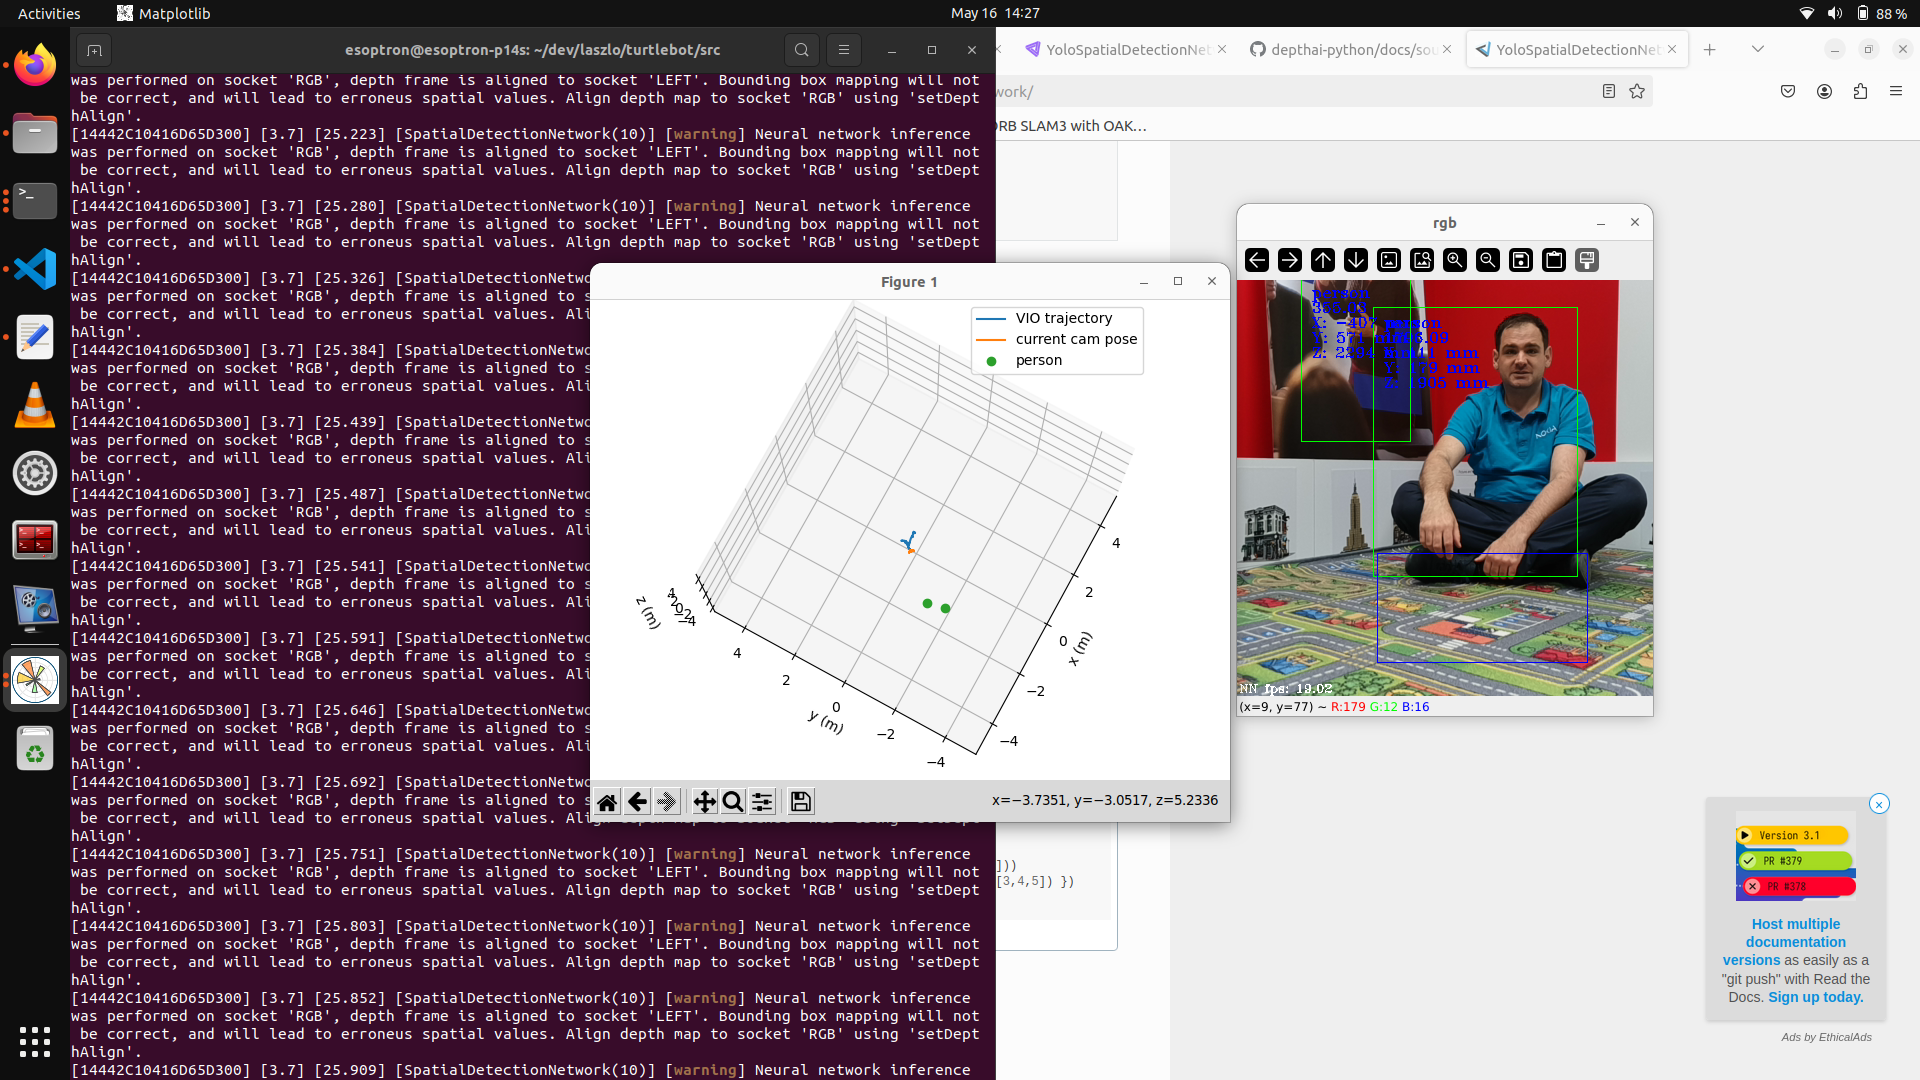
\includegraphics[width=150mm, keepaspectratio]{figures/person_detection_camera_at_front_nokia.png}
    \caption{Person detection with the camera at front at Nokia Bell Labs}
    \label{fig:person_detection_camera_at_front_nokia}
\end{figure}

After we experimented with the FOV and the example detection script I created a custom script based on the example which uses the camera to detect persons and publish their location in world coordinates on a ROS topic (the code can be examined at \ref{custom_person_detector}). It is worth mentioning that the base example (and my code too) is needed to be upgraded because after some detections it freezes with an error indicating that the IMU buffer size is exceeded. It may be because the IMU sends data too rapidly and the configuration of the \verb|SpatialLocationCalculator| node uses a buffer that is too small. Unfortunately we had no time to further investigate this issue but it seems really complex due to it lays inside the \verb|SpatialLocationCalculator| camera pipeline node.
